\documentclass[landscape,a0paper,fontscale=0.285]{baposter}

\usepackage{graphicx} % Required for including images

\usetikzlibrary{positioning}

% Font
\usepackage{palatino}
\usepackage{relsize}

% Style
\usepackage{calc}
\usepackage{enumitem}
\usepackage{multicol}
\usepackage{proof}
\usepackage{amsmath}
\usepackage{amssymb}
\usepackage{tabularx}
\usepackage{booktabs}
\usepackage{minted}
\usepackage{pifont}% http://ctan.org/pkg/pifont
\newcommand{\cmark}{\ding{51}}%
\newcommand{\xmark}{\ding{55}}%

%\definecolor{color1}{HTML}{8b0000}
\definecolor{color1}{RGB}{192,10,53}
%\definecolor{color2}{HTML}{006400}
\definecolor{color2}{RGB}{36,167,147}
\definecolor{UU-yellow}{RGB}{255,205,0}
\definecolor{UU-red}{RGB}{192,10,53}
\definecolor{UU-black}{RGB}{0,0,0}
\definecolor{UU-green}{RGB}{36,167,147}
\definecolor{UU-white}{RGB}{255,255,255}
\definecolor{UU-cream}{RGB}{250,230,171}
\definecolor{termcolor}{RGB}{0,0,0}

\newsavebox{\mintedbox}	

\setlist[itemize]{leftmargin=*}
\setlength{\columnsep}{2cm}

\include{commands}
\newcolumntype{M}{>{\centering\arraybackslash}m{\dimexpr.25\linewidth-2\tabcolsep}}


\begin{document}

\begin{poster}{
  % General options
  columns=3,
  eyecatcher=true,
  borderColor=black,
  headerFontColor=white,
  background=plain,
  bgColorOne=UU-cream!50,
  bgColorTwo=UU-yellow,
  boxColorOne=white,
  boxColorTwo=white,
  headershade=plain,
  headerColorOne=black,
  headerColorTwo=black,
  % Eyecatcher
  % eyeCatcherleft=false,
  % eyeCatcherRight=false,
  % % Header
  % headerheight=0.15\textheight,
  % headerborder=closed,
  % headershape=rectangle,
  % headershade=plain,
  % headerfont=\Large\bfseries\scshape,
  % Text box
  textborder=rounded,
  % textfont=\small,
  % textalign=left,
  % textline=2ex,
  % Box
  boxheaderheight=0.05\textheight,
  headerborder=open,
  headershape=rounded,
  % boxheaderborder=closed,
  % boxheadershape=rectangle,
  headerfont=\large\textbf,
  % Format
  % linewidth=1pt
}
{\hspace{50pt}
\includegraphics[width=0.04\textwidth]{NWO logo - zw.png}
\hspace{25pt}
{\includegraphics[width=0.25\textwidth,trim={1cm 1cm 1cm 1cm},clip]{UU_logo_2021_EN_rgb.png}}
}
{\huge Spinning Raw Text into Lambda Terms with Graph Attention}
{\Large
    Konstantinos Kogkalidis\textsuperscript{$\diamond$},
    Michael Moortgat\textsuperscript{$\diamond$},
    Richard Moot\textsuperscript{$\bx$}\\
    {\large
    {$\diamond$} Institute for Language Sciences, Utrecht University | {$\bx$} LIRMM, Universit\'{e} de Montpellier, CNRS
    }
}


% Introduction
\headerbox{Introduction}{name=intro,column=0,row=0}{
    % \begin{table}
	% \centering
	\textbf{Categorial Grammars} \& the \textbf{Holy Trinity} :\\
	
	\begin{tabularx}{0.99\textwidth}{@{}ccC@{}}
	\textbf{Logic}			& \textbf{Computer Science} 	& \textbf{Linguistics}\\
	\toprule
	Propositional Constant	& Base Type						& Syntactic Category\\
	Inference Rule			& Term Rewrite					& Phrase Formation\\
	Axiom					& Variable						& Word\\
	Provability				& Type Inhabitation	 			& Grammaticality\\
	Deduction				& Program Synthesis				& Parsing
	\end{tabularx}\vspace{1em}
	
	Standard pipeline:
	
	\hfil parse surface form $\implies$ convert to $\lambda$ $\implies$ downstream task
	
	\vspace{1em}
	This work:
	
	\hfil parse deep $\lambda$ form $\implies$ downstream task
}

% Type-logical grammars
\headerbox{Type Grammar}{name=grammar,column=0,below=intro}{
    A \textbf{semantics-first}, \textbf{type-driven} grammar for the 21st century.\linebreak
    Combines:
    \begin{enumerate}[topsep=0pt]
        \item a linear functional core
        \item a set of residuated modalities
    \end{enumerate}
    to capture:
    \begin{enumerate}[topsep=0pt]
        \item grammatical function-argument structures
        \item dependency-domain annotations (\textcolor{UU-red}{$\longleftarrow$ new fancy feature!})
    \end{enumerate}
    
    \vspace{0.5em}
   	\hfill\begin{minipage}{0.5\textwidth}
		\begin{itemize}[topsep=0pt]
			\item[\cmark] cooler than CCG!
			\item[\cmark] type checks!
		\end{itemize}
  	\end{minipage}
	\vspace{1em}

    \setlength{\abovedisplayskip}{0pt}
    \setlength{\belowdisplayskip}{0pt}
    \textbf{Grammatical Types} are inductively defined as:
    \begin{align*}
        \type{a}, \type{b} \ := \ & p                       & & \text{\# base categories, e.g. $\type{np}$} \\
                                  & | \ \ddia{d}\type{a}    & & \text{\# d-marked \textit{\textcolor{color1}{complements}}, e.g. $\ddia{su}\type{np}$} \\
                                  & | \ \type{a}\li\type{b} & & \text{\# grammatical functions, e.g. $\ddia{su}\type{np}\li\type{s}$} \\
                                  & | \ \dbox{d}\type{a}    & & \text{\# d-marked \textit{\textcolor{color2}{adjuncts}}, e.g. $\dbox{d}(\type{np}\li\type{np})$}
    \end{align*}
    \vspace{0.5em}
    
    \textbf{Inference Rules} assert grammaticality and provide recipes for compositional meaning assembly in the form of $\lambda$ expressions:\vspace{1em}
    
    \begin{tabularx}{1\textwidth}{@{}CC@{}}
        $\infer[\ax]{\term{x}: \type{a} \vdash~\textcolor{black}{\term{x}}: \type{a}}{}$
        &
        $\infer[\lex]{\term{c}: \type{a} \vdash~\textcolor{black}{\term{c}}: \type{a}}{(\term{c}\mapsto \type{a}) \in \mathcal{L}}$\\[1em]
        $\infer[\li E]{\Gamma, \Delta \vdash \textcolor{black}{\term{s~t}}: \type{b}}{\Gamma \vdash \textcolor{black}{\term{s}}: \type{a} \li \type{b} & \Delta \vdash \textcolor{black}{\term{t}}: \type{a}}$
        & 
        $\infer[\li I]{\Gamma \vdash \textcolor{black}{\term{\lambda x.s}}: \type{a} \li \type{b}}{\Gamma, \term{x}: \type{a} \vdash \textcolor{black}{\term{s}}: \type{b}}$\\[1em]
        $\infer[\dbox{\delta} E]{\dbra{\Gamma}{\textcolor{color2}{\delta}} \vdash \textcolor{black}{\bxelim[\delta]{\term{s}}}: \type{a}}{
            \Gamma \vdash \textcolor{black}{\term{s}}: \dbox{\delta}\type{a}
        }$
        &
        $\infer[\ddia{\delta} I]{\dbra{\Gamma}{\textcolor{color1}{\delta}} \vdash \textcolor{black}{\diaintro[\delta]{\term{s}}}: \ddia{\delta} \type{a}}{
            \Gamma \vdash \textcolor{black}{\term{s}}:\type{a}
        }$
    \end{tabularx}
}

\headerbox{Proof Representations}{name=st,column=1,row=0}{
  In \textbf{Natural Deduction}:\\
      \begin{tikzpicture}[t/.style={text depth=.25ex, rectangle, outer sep=3pt,align=center}]
        \node[t] (proof) at (0,0) {
            \resizebox{0.99\textwidth}{!}{
                \infer[\li E]
                    {\term{c_0}, \cbra{\term{c_1}, \cbra{\abra{\term{c_2}}{det},\abra{\term{c_3}}{mod}, \term{c_4}}{su}}{whbody} \vdash \textcolor{termcolor}{\term{c_0}~\diaintro[whbody](\lambda \term{x}.\term{c_1}~\term{x}~\diaintro[su](\bxelim[det](\term{c_2})~(\bxelim[mod](\term{c_3})~\term{c_4}))}:
 \gtype{whq}}
                    {
                        \infer[\lex]{\term{c_0}\vdash \ddia{whbody}(\ddia{predc}\gtype{pron}\li\gtype{svi})\li\gtype{whq}}{\w{What}}
                        &
                        \hspace{-85pt}
                        \infer[\ddia{whbody}I]
                        {\cbra{\term{c_1}, \abra{\abra{\term{c_2}}{det},\abra{\term{c_3}}{mod}, \term{c_4}}{su}}{whbody} \vdash \ddia{whbody}({\ddia{predc}\gtype{pron}\li\gtype{svi}})}
                        {
                            \infer[\li I]
                            {\term{c_1}, \cbra{\abra{\term{c_2}}{det},\abra{\term{c_3}}{mod}, \term{c_4}}{su} \vdash \ddia{predc}\gtype{pron}\li\gtype{svi}}
                            {
                            		\hspace{-70pt}
                                \infer[\li E]
                                {\term{c_1}, \term{x}, \cbra{\abra{\term{c_2}}{det},\abra{\term{c_3}}{mod}, \term{c_4}}{su} \vdash \gtype{svi}}
                                {
                                    \infer[\li E]
                                    {\term{c_1}, \term{x} \vdash \ddia{su}\gtype{np}\li\gtype{svi}}
                                    {
                                        \infer[\lex]
                                        {\term{c_1}\vdash \ddia{predc}\gtype{pron}\li\ddia{su}\gtype{np}\li\gtype{svi}}
                                        {\w{is}}
                                        &
                                        \infer[\ax]
                                        {\term{x}\vdash \ddia{predc}\gtype{pron}}
                                        {}
                                    }
                                    &
                                    \hspace{-10pt}
                                    \infer[\ddia{su} I]
                                    {\cbra{\abra{\term{c_2}}{det},\abra{\term{c_3}}{mod}, \term{c_4}}{su} \vdash \ddia{su}\gtype{np}}
                                    {
                                        \infer[\li E]
                                        {\abra{\term{c_2}}{det},\abra{\term{c_3}}{mod}, \term{c_4} \vdash \gtype{np}}
                                        {
                                            \infer[\dbox{det} E]
                                            {\abra{\term{c_2}}{det} \vdash \gtype{n}\li\gtype{np}}
                                            {
                                                \infer[\lex]
                                                {\term{c_2}\vdash \dbox{det}(\gtype{n}\li\gtype{np})}
                                                {\w{that}}
                                            }
                                            &
                                            \infer[\li E]
                                            {\abra{\term{c_3}}{mod}, \term{c_4} \vdash \gtype{n}}
                                            {
                                                \infer[\dbox{mod} E]
                                                {\abra{\term{c_3}}{mod} \vdash \gtype{n}\li\gtype{n}}
                                                {
                                                    \infer[\lex]
                                                    {\term{c_3}\vdash \dbox{mod}(\gtype{n}\li\gtype{n})}
                                                    {\w{scary}}
                                                }
                                                &
                                                \infer[\lex]
                                                {\term{c_4}\vdash \gtype{n}}
                                                {\w{figure}}
                                            }
                                        }
                                    }
                                }
                            }
                        }
                    }
                }
    	    };
    	    \node[t] (dep) at ($(proof.south) + (0, -1)$) {
    	        \resizebox{110pt}{!}{
                \begin{tikzpicture}
                \node[t] (wat) 			at (0, 0) {\w{What}};
                \node[t] (is)		    [right=10pt of wat] {\w{is}};
                \node[t] (dat) 			[right=10pt of is] {\w{that}};
                \node[t] (rare) 	    [right=10pt of dat] {\w{scary}};
                \node[t] (tekening)		[right=10pt of rare] {\w{figure}};
                \draw[->,color=color1] (wat)         [bend left=60] edge node [above] {\smaller[2]{whbody}} (is);
                \draw[->,color=color1] (is)          [bend left=90] edge node [above] {\smaller[2]{su}} (tekening);
                \draw[->,color=color2] (tekening)      [bend right=30] edge node [above] {\smaller[2]{mod}} (rare);
                \draw[->,color=color2] (tekening)      [bend right=70] edge node [above] {\smaller[2]{det}} (dat);
                \end{tikzpicture}
                }
            };
	    \end{tikzpicture}\vspace{1em}
	    
\hfill\begin{minipage}{0.9\textwidth}
	    a \textbf{proof-tree}
	    \begin{itemize}[topsep=0pt,leftmargin=20pt]
	    		\item[\cmark] clear computational interpretation
	    		\item[\cmark] trivial interface to a dependency tree
	    		\item[\cmark] correct by construction
	    		\item[\xmark] takes time to build (induction in \textit{depth})
	    		\item[\xmark] odd structure for ML (can't batch!)
	    \end{itemize}
	    \end{minipage}
	    

\vspace{2em}
As a \textbf{Proof Net}:\\
	\begin{center}
	\resizebox{0.9\textwidth}{!}{
		\begin{tikzpicture}
		    [t/.style={text height=1.5ex, text depth=.25ex, rectangle, outer sep=5pt}, node distance=10pt,
		    r/.style={text=color1},
		    g/.style={text=color2},
		    tree/.style={very thick},
		    link/.style={dashed}]
		\node[t] (wat)      at (0, 0) {\w{What}};
		\node[t,g] (wat_fn_1) at (0, 1) {$\li\ddia{whbody}$};
        \node[t,r] (wat_fn_2) at (-1.5, 2.5) {$\li\ddia{predc}$};
        \node[t, g] (wat_pron) at (-2.5, 4) {$\type{pron}^0$};
        \node[t, r] (wat_svi) at (-0.5, 4) {$\subcat{s}{s}{vi}^1$};
        \node[t, g] (wat_whq) at (1.5, 2.5) {$\type{whq}^2$};

		\node[t] (is) at (4, 0)     {\w{is}};
		\node[t,g] (is_fn_1) at (4, 1)  {$\li\ddia{predc}$};
		\node[t,g] (is_fn_2) at (5, 2.5) {$\li\ddia{su}$};
		\node[t,r] (is_pron) at (3, 2.5) {$\type{pron}^3$};
		\node[t,r] (is_np) at (4.25, 4) {$\type{np}^4$};
		\node[t,g] (is_svi) at (5.75, 4) {$\subcat{s}{s}{vi}^5$};
		
		\node[t] (dat)   at (8, 0)   {\w{that}};
		\node[t,g] (dat_fn) at (8, 1)  {$\dbox{det}\li$};
		\node[t,r] (dat_n) at (7, 2.5) {$\type{n}^6$};
        \node[t,g] (dat_np) at (9, 2.5) {$\type{np}^7$};
        
        \node[t] (rare)   at (11, 0)   {\w{scary}};
		\node[t,g] (rare_fn) at (11, 1)  {$\dbox{mod}\li$};
		\node[t,r] (rare_n_1) at (10, 2.5) {$\type{n}^8$};
        \node[t,g] (rare_n_2) at (12, 2.5) {$\type{n}^9$};	
        
        \node[t] (tekening) at (14, 0) {\w{figure}};
        \node[t,g] (tekening_n) at (14, 1) {$\type{n}^{10}$};

        \draw[tree] (wat_fn_1) -- (wat_fn_2) -- (wat_pron);
        \draw[tree] (wat_fn_2) -- (wat_svi);
        \draw[tree] (wat_fn_1) -- (wat_whq);
        
        \draw[tree] (is_fn_1) -- (is_pron);
        \draw[tree] (is_fn_1) -- (is_fn_2) -- (is_np);
        \draw[tree] (is_fn_2) -- (is_svi);
        
        \draw[tree] (dat_fn) -- (dat_n);
        \draw[tree] (dat_fn) -- (dat_np);
        
        \draw[tree] (rare_fn) -- (rare_n_1);
        \draw[tree] (rare_fn) -- (rare_n_2);

        \draw[->, dashed] (tekening_n) -- ($(tekening_n) + (0, 2.5)$) -| (rare_n_1);
        \draw[->, dashed] (rare_n_2) -- ($(rare_n_2) + (0, 1.5)$) -| (dat_n);
        \draw[->, dashed] (dat_np) -- ($(dat_np) + (0, 2.5)$) -| (is_np);
        \draw[->, dashed] (is_svi) -- ($(is_svi) + (0, 1.5)$) -| (wat_svi);
        \draw[->, dashed] (wat_pron) -- ($(wat_pron) + (0, 0.75)$) -| (is_pron);
        \draw[->, dashed] (wat_whq) -- ++ (0, 4);
	    \end{tikzpicture}
	   }
	  \end{center}
	  
	 \hfill\begin{minipage}{0.9\textwidth}
	    a \textbf{proof-graph}
	    \begin{itemize}[topsep=0pt,leftmargin=20pt]
	    		\item[\cmark] each type decomposed to a bicolor tree
	    		\item[\cmark] functional relations specified as a bijection
	    		\item[\cmark] fully parallel, easy to vectorize
	    		\item[\xmark] computationally intractable ($n!$ combinations)
	    		\item[\xmark] requires formal verification 
	    \end{itemize}
	    \end{minipage}
	
	\begin{center}    
	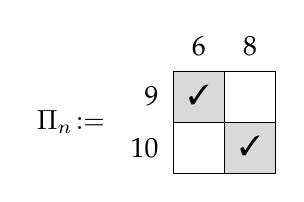
\begin{tikzpicture}[scale=.65]
	    \fill[gray!30] (0,1) rectangle +(1,1);
	    \node [above] at (0.5, 1.15) {\cmark};
	    \fill[gray!30] (1,0) rectangle +(1,1);
	    \node [above] at (1.5, 0.15) {\cmark};
	    \node [above] at (0.5,2.1) {6};
	    \node [above] at (1.5,2.1) {8};
	    \node [left] at (-0.1,1.5) {9};
	    \node [left] at (-0.1,0.5) {10};
	    \node at (-2,1) {${\Pi}_\type{n}\!:=$};
	    \draw (0,0) grid (2,2);
	\end{tikzpicture}\hphantom{1500000}
	\end{center}
}

  % System Architecture
\headerbox{System Architecture}{name=architecture,column=2,row=0}{
 	{\larger spind\textsuperscript{2}$\lambda$e}
 	\hrule
 	
 	\hfill\underline{s}pind\textsuperscript{2}$\lambda$e \underline{p}arses \underline{in}to \underline{d}ependency-\underline{d}ecorated \underline{$\lambda$} \underline{e}xpressions
 	
 	\vspace{1em}
 	A neat packaging of:
  	\begin{itemize}[itemsep=5pt,topsep=0pt,leftmargin=15pt]
  		\item[1.] \textbf{a graph-based supertagger}
  		\begin{itemize}[topsep=0pt]
			\item[i.] learns (word $\mapsto$ type) mapping as a \textcolor{UU-red}{graph generation task}
			\item[ii.] can correctly produce \textcolor{UU-red}{new} types on demand
			\item[iii.] \textcolor{UU-red}{SOTA} across datasets (multi-framework, multi-lingual)
			\item[iv.] length-parallel, depth-linear decoding (i.e. \textcolor{UU-red}{constant})
  		\end{itemize}
  		\item[2.] \textbf{an OT-based proof search module}
		\begin{itemize}[topsep=0pt]
			\item[i.] learns proof search as a \textcolor{UU-red}{node matching task}
			\item[ii.] \textcolor{UU-red}{fully parallel} in batch/depth/length
			\item[iii.] \textcolor{UU-red}{no iteration} (unlike shift-reduce)
	 	\end{itemize}
	 	\item[3.] \textbf{a mini type checker}
	 	\begin{itemize}[topsep=0pt]
			\item[i.] Python DSL to write/manipulate well-typed parses
			\item[ii.] handles proof net $\longleftrightarrow$ nat. ded. $\longleftrightarrow$ $\lambda$-term conversions
			\item[iii.] asserts validity of neural output
			\item[iv.] user-friendly hooks
	 	\end{itemize}
	 \end{itemize}
}

\headerbox{Experiments}{name=res,column=2,below=architecture}{
\textbf{Current implementation} trained/evaluated on \AE thel ($\sim$70,000 proof-derivations of written Dutch):

	\vspace{0.5em}
	{\smaller
	\hfil\begin{tabular}{@{}c@{\qquad}c@{}}
			\textbf{parsability}	&
			\textbf{coverage} \\
			\smaller(some proof obtainable) &
			\smaller(some proof obtained) \\
			\toprule
			86.83 &
			84.94 \\
			\addlinespace
			\textbf{types correct} &
			\textbf{accuracy}\\
			\smaller(correct proof obtainable) & 
			\smaller(correct proof obtained)\\
			\toprule
			56.88 & 
			{55.30}\\
		\end{tabular}
	}
	
	\vspace{0.5em}	
	\hfill\begin{minipage}{0.95\textwidth}
	    \begin{itemize}[topsep=0pt,leftmargin=20pt]
    	    		\item faster \& stricter than conventional parsers, just as accurate
	    		\item proof search bottlenecked by supertagging
	    \end{itemize}
	    \end{minipage}
}

\headerbox{Try It Out/Read More}{name=test,column=2,below=res}{
	
	\begin{center}
	\begin{tabular}{@{} >{\centering\arraybackslash} m{2cm} >{\centering\arraybackslash} m{3.72cm}@{}}
		
\includegraphics[width=0.15\textwidth]{qr-code.png} & source code, installation instructions \& usage examples \\
		
\includegraphics[width=0.15\textwidth]{arxiv-qr.png} & arXiv preprint
	\end{tabular}

%		
	\end{center}
}

\end{poster}

\end{document}
